%; whizzy paragraph -pdf xpdf -latex ./whizzypdfptex.sh
%; whizzy-paragraph "^\\\\begin{frame}\\|\\\\emtext"
% latex beamer presentation.
% platex, latex-beamer でコンパイルすることを想定。 

%     Tokyo Debian Meeting resources
%     Copyright (C) 2012 Junichi Uekawa
%     Copyright (C) 2011 Nobuhiro Iwamatsu

%     This program is free software; you can redistribute it and/or modify
%     it under the terms of the GNU General Public License as published by
%     the Free Software Foundation; either version 2 of the License, or
%     (at your option) any later version.

%     This program is distributed in the hope that it will be useful,
%     but WITHOUT ANY WARRANTY; without even the implied warreanty of
%     MERCHANTABILITY or FITNESS FOR A PARTICULAR PURPOSE.  See the
%     GNU General Public License for more details.

%     You should have received a copy of the GNU General Public License
%     along with this program; if not, write to the Free Software
%     Foundation, Inc., 51 Franklin St, Fifth Floor, Boston, MA  02110-1301 USA

\documentclass[cjk,dvipdfmx,12pt]{beamer}
\usetheme{Tokyo}
\usepackage{monthlypresentation}

%  preview (shell-command (concat "evince " (replace-regexp-in-string "tex$" "pdf"(buffer-file-name)) "&")) 
%  presentation (shell-command (concat "xpdf -fullscreen " (replace-regexp-in-string "tex$" "pdf"(buffer-file-name)) "&"))
%  presentation (shell-command (concat "evince " (replace-regexp-in-string "tex$" "pdf"(buffer-file-name)) "&"))

%http://www.naney.org/diki/dk/hyperref.html
%日本語EUC系環境の時
\AtBeginDvi{\special{pdf:tounicode EUC-UCS2}}
%シフトJIS系環境の時
%\AtBeginDvi{\special{pdf:tounicode 90ms-RKSJ-UCS2}}

\title{大統一Debian勉強会}
\subtitle{U-Bootについてあれこれ}
\author{野島 貴英\\nozzy@debian.or.jp}
\date{2012年6月13日}
\logo{
\includegraphics[width=8cm]{image200607/openlogo-light.eps}}

\begin{document}

\frame{\titlepage{}}

\begin{frame}{自己紹介}

\begin{itemize}
\item Linuxは長年触ってます(でも詳しくない...orz)
\item Linuxとの付き合いは組み込み用途の安価なOSとしてMSDOS以外でOS探してたのが動機といえば動機。
\item ITの波に飲まれて、今はIT系のサーバー屋。でもCloud時代もきちゃって仕事なくなりそうなので、次は何しようかなぁーと模索中。
\end{itemize}

\end{frame}

\begin{frame}{ところでみなさん組み込みシステムって知ってますかー?}

組み込みシステムとは:\\
「特定の機能を実現するためのコンピュータシステムの事」\\
だそうで...
\begin {itemize}
\item 特定の機能を実現できれば良いので、部品削ってケチりまくる事多数。
\item 一方で、極端にタフな動作環境、動作が求められます
\item 特定の機能を実現の為、妙な入出力センサ沢山搭載してます
\end{itemize}

\end{frame}

\begin{frame}{組み込みシステムのプロの方いますー?}

\begin{itemize}
\item プロの方が過半数越えた場合:プランA(BOF、アドリブ多め)
\item プロの方が過半数未満の場合:プランB(資料を元に...)
\end{itemize}

\end{frame}

\begin{frame}{どんなCPU使ってます?}

差し支え無い範囲で教えていただけますと嬉しいな...

\begin{itemize}
\item SHシリーズ?
\item ARM?
\item PIC系?
\item Intel x86系?
\item Z80?
\item Motrora 68000系?
\item PowerPC?
\item その他
\end{itemize}

\end{frame}

\begin{frame}{今回の発表はARM機材で}

巷でARM流行ってるよね?

\begin{itemize}
\item 昨今のスマホ事情、Android端末などの関係で、いろいろ評価ボードの入手が便利。
\item 電子書籍端末もARMベースだったり(今回のターゲットボード)
\item Rasberry Piも(入荷状況は混雑しまくりの模様ですが...)
\end{itemize}

 というわけで、今回の発表は妙にARM CPUに偏ります。他のCPUの話
を聞きたい方はすみませんが、情報交換をさせていただければ嬉しいな。

 ※他の評価機材を自分は持っていない事は秘密です。

\end{frame}

\begin{frame}{今回SoCはTexas Instrumentsで}

自分の趣味ですが、「ありがとう!TI子供の時からファンだったよ!」\\
(74シリーズとか。当時7セグドライバから始まり...大人になってはDSP...)\\

良いところ\\
\begin{itemize}
\item サポートとコミュニティが諸々ある。
\item いろいろオープンにしてくれてる(エコシステムとの事)
\item 流行りのチップいろいろのっけてる(VRシリーズのOpenGL ESアクセラレーションつきGraphicsチップとか)
\end{itemize}

なので、実機のSoCはOMAP36シリーズにて。

\end{frame}


\begin{frame}{自分の家でも組み込みやってます?}

差し支え無い範囲で教えていただけますと嬉しいな...

\begin{itemize}
\item ICE持ってます?
\item ロジアナある?
\item オシロある?
\end{itemize}

\end{frame}

\begin{frame}{ところでブートローダ}

外部記憶装置に搭載したOSを主記憶へ展開して、実行を引き継ぐ為のシンプルなソフトウェア。

でも昨今は、
\begin{itemize}
\item スクリプト言語は積むわ、
\item 様々な外部記憶装置にアクセスするために、数々のチップセットの制御コードを搭載するわ、
\item 数々のフォーマット/ファイルシステムに対応するようになるわ、
\item インタラクティブにユーザとやりとりする為の簡易デバッガ(リモートデバッグの為のドライバも含む)、モニタなど積むわ、
\end{itemize}

など、シンプルだった「はず」のソフトウェアは機能強化の道をひた走る...

\end{frame}

\begin{frame}{主なブートローダ一覧}

Comparison of boot loaders\\
\url{http://en.wikipedia.org/wiki/Comparison_of_boot_loaders}

そりゃもういろいろある模様。

\end{frame}

\begin{frame}{U-Boot}

 DENX Software Engineering社が主にメンテしているGPLなブートローダの実装。
 \begin{itemize}
  \item 今ではDas U-Bootといったりもします。
  \item 先の''Comparison of boot loaders''にあるとおり、圧倒的な量のサポートCPU数を誇る。
  \item モニタ、デバッガスタブ、独自のスクリプト言語を搭載
  \item ブート対象のOSはLinuxに偏ってるかな...
 \end{itemize}

\end{frame}

\begin{frame}{百聞は一見にしかず}

百聞は一見にしかず。まずversatilepbエミュレータで動作させて試してみます。
(...やり方は書くと長いので、大統一Debian勉強会資料を参照...)

QEMUのおかげで、ブートからシミュレーションも一発さ!
\end{frame}

\begin{frame}{え?やり方分かりにくいって?}
大統一Debian勉強会資勉強会資料のやり方を図示するとわかりやすいです。
※全部で4ページの制約がありまして割愛しちゃいました...ごめん

\begin{center}
  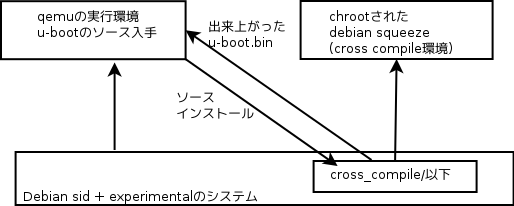
\includegraphics[width=1.0\hsize]{image2012-gum/u-boot-cross-diagram.png}
\end{center}


\end{frame}

\begin{frame}{補足:ところでversatilepbって何}

ARM社の評価ボードVERSATILEシリーズの1つ。
\url{http://www.arm.com/ja/products/tools/development-boards/versatile/platform-baseboards.php}

CPUはARM926EJ-S。

感想:本物は触ってないので実際はどうかは未評価。QEMUではHDDデバイス、PCIデバイス、ネットまでつながる素敵な奴。debianのARM版試したりするのに最高(東京エリアDebian勉強会資料「Deb専」2012/04月参照)メモリを512MBytes以上にQEMUで設定するとカーネルがなぜか死ぬけど...(なぜだ?)

\end{frame}

\begin{frame}{補足その2:なんでexperimentalのqemuなのか?}

なんでわざわざexperimental版qemuなの?

理由:\\
\url{http://www.elinux.org/Virtual_Development_Board}
のパッチが当たっているバージョンのQEMUが必要な為です。実際デバッガ回しながら
QEMU追いかけるとわかるのですが、versatilepb版のU-Bootがpflashの初期化をしようと
すると、QEMU側のversatilepbエミュレーションにそれを受け入れるコードが無い為、
exceptionを発生してしまい停止します。

\end{frame}

\begin{frame}{U-Boot初めて触る人には簡単なコマンド}

\begin{itemize}
\item help\\
helpのみで一覧。あとはhelp コマンド名でhelpが読める。
\item bdinfo\\
ボードの情報を表示。
\item printenv \\
環境変数(いじるといろいろU-Bootの動作を変えられる)
\item setenv \\
環境変数いじってみる。
\end{itemize}

\end{frame}

\begin{frame}{ところでU-Boot便利}

自分から見た良いところ

\begin{itemize}
\item LCD/Flash/USBとかの出力デバイスなど共通/便利/必要そうなものは共通化されている。
\item 数々のファイルシステムに対応(cramfs/ext2/fat/jffs2/reiserfs...等)
\item 設定ファイル(というか設定バイナリ)である程度作を変更可能
\item LCDについてはフォントすら内臓してるのでラスタ形式のビットマップしかLCDに描画できなくても余裕。
\item 基本設計は変に複雑でないところ(抽象化やりすぎとかがないので...。)また、沢山のわかりやすいマクロとスイッチ。
\end{itemize}

\end{frame}

\begin{frame}{U-Bootを俺ボードで動かす時は(初心者向け1/2)}

\begin{itemize}
\item Step1. \\
u-boot-src/READMEを読む
\item Step2.\\
CPU/SoCがu-boot-src/arch以下にすでにあれば再利用を検討
\item Step3. \\
ボードのチップセット/回路が近いものがあれば、u-boot-src/board/以下をパクる
\item Step4. \\
u-boot-src/include/configs以下に対応したファイルを作成し、U-Bootの数々のマクロ定数を定義する。
\end{itemize}

\end{frame}

\begin{frame}{U-Bootを俺ボードで動かす時は(初心者向け2/2)}

\begin{itemize}
\item Step5. u-boot-src/boards.cfgに俺ボードに対応した定義を入れてやり、Step1/Step2/Step3を融合する。
\end{itemize}

で、あとはmake ARCH=XXX CROSS\_COMPILE=gccのクロスコンパイル用コマンドのprefix 俺ボード名\_configしてmake。(「俺ボード名」の部分はu-boot-src/boards.cfgに記載した名前)

ただし、最近はfdt(Flatten Device Tree)とか便利なものもあるらしい。

\end{frame}


\begin{frame}{実機にBN Nook Colorを使ってみる}

これは電子書籍端末。

スペック\\
\begin{itemize}
\item SoCにはOMAP36シリーズを利用
\item LCD/miniSDカード/USB搭載
\end{itemize}

実はOMAP用ブート形式のフォーマットでminiSD用意して、差し込んで電源ONすると
思わずそちらからブートしちゃうという特典機能あり。

\end{frame}

\begin{frame}{BNの公開しているU-Bootソースを改造}

ただ動かすだけではまったくつまらんので、改造をしてみる。

とりあえず、LCDに
\begin{itemize}
\item カラーパターンだしてみる。
\item U-Bootメッセージ出してみる
\end{itemize}

\end{frame}

\begin{frame}{改造解説}

とりあえず勉強会資料のパッチを見てもらえばわかりやすいかと。

\begin{itemize}
\item lcd.cいじっているのは、Nook Colorの場合、起動画像(ビットマップ)を出して細かい事をかくしているのを解除する為。パッチの変更箇所下にあるlcddev.putc/lcddev.putsの変数はC分かる人にはお馴染みの関数(putc/puts)に見えますでしょうか?
\item omap3621\_evt1a.hは、stdout/stderrを全部LCDへ振り向ける環境変数を新たに定義し、さらに入出力デバイスは環境変数の中身を優先して使ってくれというマクロをONにする。
\item ついでに「カラーパターンだしてね」という内容と、「初期化時もLCD出しっぱなしにしてね」というマクロをONにする。
\item{itemize}
\end{itemize}
ほら改造も簡単。

\end{frame}

\begin{frame}{動作しました!}

\begin{center}
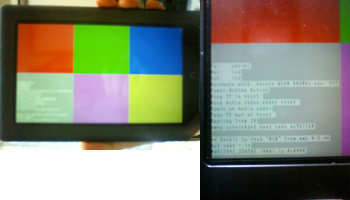
\includegraphics[width=1\hsize]{image2012-gum/u-boot-nook.png}
\end{center}

\end{frame}

\begin{frame}{最後に:Flatten Device Treeについて}

以下が参考になるかと
\begin{itemize}
\item FDTWiki\\
\url{http://devicetree.org/Main_Page}
\item ePAPR \\
\url{http://www.power.org/resources/downloads/Power_ePAPR_APPROVED_v1.0.pdf}
\end{itemize}

\end{frame}
\end{document}

;;; Local Variables: ***
;;; outline-regexp: "\\([ 	]*\\\\\\(documentstyle\\|documentclass\\|emtext\\|section\\|begin{frame}\\)\\*?[ 	]*[[{]\\|[]+\\)" ***
;;; End: ***
